\documentclass[
	fontsize=10pt,
	open=right,
	twoside,
    english,
    draft,
	%final
]{scrbook}
\usepackage[utf8]{inputenc}
\usepackage[italian,main=english]{babel}

\usepackage{showkeys}

% TODO Setup typography (fonts, mparhack, microtype...)
%\input{config/typographyConfig}
\renewcommand{\sfdefault}{iwona}

% Define some useful colors
\usepackage[dvipsnames]{xcolor}

% Define some colors
\definecolor{webgreen}{rgb}{0,.5,0}
\definecolor{webbrown}{rgb}{.6,0,0}
\definecolor{Maroon}{cmyk}{0, 0.87, 0.68, 0.32}
\definecolor{RoyalBlue}{cmyk}{1, 0.50, 0, 0}

% Setup plots
\usepackage{pgfplots}
\pgfplotsset{compat=newest}
\pgfplotsset{
    grid = major,
    major grid style={densely dotted},
    enlargelimits=.05,
    width = .75\textwidth
}
\usepgfplotslibrary{
    fillbetween,
    colormaps,
    units
}

\usepgfplotslibrary{external}
\tikzexternalize%[prefix=TikZ_pictures/]

\usepackage{tikz}
\usepackage{tikz-uml} % For UML diagrams

\usetikzlibrary{
    calc,
    shapes
}
\tikzset{>=stealth,}
\pgfplotsset{
    phase_plot/.style={%
        yticklabel style={sloped like y axis},%
        xlabel = {Mass of the final-state $\Ppiplus\Ppiminus$ system $[\si{\giga\electronvolt/\square\c}]$},
        %x unit = {\si{\giga\electronvolt/\square\c}},
        ylabel = {Dynamic-shape phase $[\si{deg}]$},
        %y unit = {\si{deg}}
    },
    amplitude_plot/.style={%
        yticklabel style={sloped like y axis},%
        xlabel = {Mass of the final-state $\Ppiplus\Ppiminus$ system $[\si{\giga\electronvolt/\square\c}]$},
        %x unit = {\si{\giga\electronvolt/\square\c}},
        ylabel = {Dynamic-shape magnitude $[\si{1\per(\giga\electronvolt/\square\c)^2}]$},
        %y unit = {\si{1\per(\giga\electronvolt/\square\c)^{-2}}}, % misaligns the plots
    },
    fit/.style={%
        mark options={%
            mark size=.75,%
            color=Maroon,%
            mark=*%
        },%
        ybar interval,%
        color=ForestGreen,%
        fill=LimeGreen,%
        fill opacity=.3,%
        % -- error bars --------
        error bars/y dir=both,%
        error bars/y explicit,%
        error bars/error bar style={color=Maroon},%
    },%
    guess/.style={%
        line width=.6,
        color=blue,
        mark=none,
        %mark options={%
        %    mark size=.75,
        %    mark=square*%
        %},%
    },%
    dalitz_plot/.style={%
        yticklabel pos=right,
        view={0}{90},%
        xlabel = {$m_{\Ppiplus\Ppiminus}^2$ $[\si{\giga\electronvolt^2\!/\c^4}]$},%
        ylabel = {$m_{\Ppiplus\Ppiminus}^2$ $[\si{\giga\electronvolt^2\!/\c^4}]$},%
        %x unit = {\si{\giga\electronvolt^2\!/\c^4}},%
        %y unit = {\si{\giga\electronvolt^2\!/\c^4}},%
        %colormap/viridis high res,%
        %colormap/winter,%
        colorbar left=true,%
        colorbar left/.append style={%
            yticklabel style={sloped like x axis},%
        },%
        %axis equal,%
    },%
    dalitz/.style={%
        scatter,%
        scatter src=z,%
        only marks,%
        mark options={%
            mark=square*,%
            mark size=1.1,%
        }%
    }%
}


% Setup units
\usepackage{siunitx}

\sisetup{
%	range-phrase=$-$,
	separate-uncertainty,
%	input-decimal-marker={.},
	output-decimal-marker={.},
	exponent-product = \cdot,
}

% Additional units

\usepackage{eurosym}
\DeclareSIUnit{\EUR}{\text{\euro{}}}
\DeclareSIUnit{\c}{\text{c}}

% Setup math
\usepackage{amsmath}

% For \ltrans
\usepackage{leftidx}

% Load constants
% Some useful math constants

% Euler number
\newcommand{\eu}{\ensuremath{\mathrm{e}}}
% Imaginary unit
\newcommand{\iu}{\ensuremath{\mathrm{i}}}

% Load delimiters
% Delimiters

% Among other tools, define DeclarePairedDelimiter
\usepackage{mathtools}

% Absolute value |-|
\DeclarePairedDelimiter{\abs}{\lvert}{\rvert}
% Norm ||-||
\DeclarePairedDelimiter{\norm}{\lVert}{\rVert}

% For \Set, \bra, \ket and so on
\usepackage{braket}

% Custom parentheses
\DeclarePairedDelimiter{\roundB}{(}{)}
\DeclarePairedDelimiter{\squareB}{[}{]}
\DeclarePairedDelimiter{\curlyB}{\{}{\}}

% Mean <.>
\DeclarePairedDelimiter{\mean}{\langle}{\rangle}

% Load numbersets
% Numbersets

% To enable \mathbb
% Also enables \Cap, \Box, \Diamond and so on
\usepackage{amssymb} % loads amsfonts

% Numbersets ------------------------
\newcommand{\numberset}[1]{\ensuremath{\mathbb{#1}}}
\newcommand{\N}{\numberset{N}}
\newcommand{\Z}{\numberset{Z}}
\newcommand{\Q}{\numberset{Q}}
\newcommand{\R}{\numberset{R}}
\newcommand{\I}{\numberset{I}}
\newcommand{\C}{\numberset{C}}
% Euclidean space
\newcommand{\E}{\numberset{E}}
% -----------------------------------

% Empty set
\newcommand{\0}{\ensuremath{\varnothing}}
% Cartesian product
\newcommand{\x}{\ensuremath{\times}}

% Load operators
% Operators

% Differential operators ------------
\newcommand{\de}{\mathop{}\!\textup{$\partial$}}
\newcommand{\uD}{\mathop{}\!\textup{$\Delta$}}
\newcommand{\ud}{\mathop{}\!\textup{d}}
\newcommand{\V}{\mathop{}\!\nabla}
\newcommand{\VV}{\ensuremath{\V^2}}
% D'Alembert operator
\newcommand{\dal}{\ensuremath{\mathop{}\!\Box}}
% -----------------------------------

% Algebra ---------------------------
\DeclareMathOperator{\tr}{tr}
\DeclareMathOperator{\diag}{diag}
% -----------------------------------

% Statistics ------------------------
\DeclareMathOperator{\erf}{erf}
\DeclareMathOperator{\cov}{cov}
% -----------------------------------


% Vectors
\usepackage{bm}
\renewcommand{\vec}[1]{\ensuremath{\mathbf{{#1}}}}

\newcommand{\A}{\ensuremath{\mathcal{A}}}
\newcommand{\package}[1]{\textsf{#1}}
\newcommand{\ROOT}{{\footnotesize{ROOT}}}
\newcommand{\MINUIT}{{\footnotesize{MINUIT}}}
\newcommand{\cpp}[1][]{{\footnotesize{C++\ifthenelse{\equal{#1}{}}{}{#1}}}}

% Setup listings
\usepackage[
    final
]{listings}
\lstset{
    language={[11]C++},%
    basicstyle=\ttfamily,%
    tabsize=4,%
    keywordstyle=\color{blue!50!black}\fontseries{b}\selectfont,%
    morekeywords={
        BreitWigner,%
        DataAccessor,%
        DataIterator,%
        DataPartition,%
        DataPoint,%
        DecayChannel,%
        DecayingParticle,%
        FinalStateParticle,%
        Flatte,%
        FlatteChannel,%
        HelicityFormalism,%
        MassBin,%
        MassShape,%
        MassShapeWithNominalMass,%
        Model,%
        Parameter,%
        Particle,%
        ParticleCombination,%
        ParticleFactory,%
        PoleMass,%
        PositiveRealParameter,%
        RealCachedValue,%
        RelativisticBreitWigner,%
        StaticDataAccessor,%
        ZemachFormalism,%
        shared_ptr,%
        unique_ptr,%
        vector,%
    },
    keywords=[2]{std, yap},% namespaces
    keywordstyle=[3]{\color{green!60!blue}\fontseries{b}\selectfont},%
    keywords=[3]{make_shared, make_unique, static_pointer_cast, complex, polar},% std-functions
    keywordstyle=[2]{\color{green!60!red}\fontseries{b}\selectfont},%
    keywords=[4]{calculate, addParameter, free_amplitude, setFinalState, lock, addInitialState, quantumNumbers, rad, addWeakDecay, addStrongDecay, create, to, read_pdl_file, add},% yap functions
    keywordstyle=[4]{\color{green!60!red}\fontseries{b}\selectfont},%
    commentstyle=\color{darkgray!80},%
    stringstyle=\color{orange!50!black},%
    frame=l,%
    numbers=left,%
    stepnumber=5,%
    numberstyle=\tiny\color{black!80},%
    escapeinside={£!}{!£},%
    %backgroundcolor=\color{cyan!10},%
}



% Setup index
% COnfiguration file for the index

\usepackage{makeidx}
\usepackage{multicol}

% enable generation of index via '\printindex' command in the document environment
\makeindex

%%
\let\orgtheindex\theindex
\let\orgendtheindex\endtheindex
\def\theindex{%
	\def\twocolumn{\begin{multicols}{2}}%
	\def\onecolumn{}%
	\clearpage
	\orgtheindex
}
\def\endtheindex{%
	\end{multicols}%
	\orgendtheindex
}
%%%%%%%%%%%%%%%%%%%%%%%%%%%

% Setup bibliography
% Setup bibliography
\usepackage[
	backend=biber,
]{biblatex}
\usepackage{csquotes}
\addbibresource{backmatter/bibliography.bib}


% Define abstract environment for *book class
% Define the abstract environment in a book (or scrbook) documentclass
%\usepackage{fancyhdr}
%\newcommand{\fncyblank}{\fancyhf{}}
\newenvironment{abstract}%
{\cleardoublepage\thispagestyle{empty}\null\vfill\begin{center}%
\bfseries\abstractname\end{center}}%
{\vfill\null}

% Define acknowledgements environment
% XXX Load _after_ abstractConfig.tex!!
% Define the acknowledgements environment in a book (or scrbook) documentclass

% These are already loaded/defined in abstractConfig.tex
%\usepackage{fancyhdr}
%\newcommand{\fncyblank}{\fancyhf{}}

\newenvironment{acknowledgements}%
{\cleardoublepage\fncyblank\null\vfill\begin{center}%
\bfseries{Acknowledgements}\end{center}}%
{\vfill\null}


% Setup hyperref
% Setup hyperref
\usepackage{hyperref}
\hypersetup{
    %draft,
    final,
    %colorlinks=false,
    colorlinks=true,
    linktocpage=true,
    pdfstartpage=3,
    pdfstartview=FitV,
    breaklinks=true,
    pdfpagemode=UseNone,
    pageanchor=true,
    pdfpagemode=UseOutlines,%
    plainpages=false,
    bookmarksnumbered,
    bookmarksopen=true,
    bookmarksopenlevel=1,%
    hypertexnames=true,
    pdfhighlight=/O,
    urlcolor=webbrown,
    linkcolor=RoyalBlue,
    citecolor=webgreen,
%   pagecolor=RoyalBlue,%
}

% Setup acronyms
% XXX Load it _after_ hyperref, babel, polyglossia, inputenc and fontenc
% For acronyms (and glossaries)
\usepackage[
	makeindex,% use this to make gloxary
	acronym,%
	nomain,% suppress the main (default) glossary
	hyperfirst=false, % no hyperlink at first use of acronym
	toc,% add voice in toc
]{glossaries} % XXX Load it _after_ hyperref, babel, polyglossia, inputenc and fontenc

\usepackage{relsize} % defines \textsmaller{} used by the following style
\setacronymstyle{long-sm-short}

\makenoidxglossaries


% Define acronyms
\newacronym{cuda}{CUDA}{Compute Unified Device Architecture}


% Add this package to draw molecules (needed for the caffeine!)
\usepackage{chemfig}
% Change atom font in molecule figures
\renewcommand*\printatom[1]{\ensuremath{\mathsf{#1}}}

\usepackage[
%    notitalic, % particle names are upright
%    maybess,  % allow sans serif if surrounding is sans serif
]{hepnames}
\usepackage{pgfplots}
\pgfplotsset{compat=1.14}
\usepgfplotslibrary{fillbetween}
\usepgfplotslibrary{external}
%\tikzexternalize
\usetikzlibrary{calc}
\tikzset{>=stealth,}
\usepackage{lipsum}
\usepackage{qrcode}

\title{}
\subtitle{}
\author{
  \input{AUTHORS}
}
\date{}

\begin{document}

%----------------------------------------------------------------------------------------
% FRONTMATTER
%
\frontmatter
\pdfbookmark[0]{Title}{chap:title}
	\maketitle
	\thispagestyle{empty}

	\cleardoublepage
\pdfbookmark[0]{Dedication}{chap:dedication}
	\thispagestyle{empty}
    \null\vspace{\stretch {1}}
        \begin{flushright}
                This is the Dedication.
        \end{flushright}
\vspace{\stretch{2}}\null


	\cleardoublepage
\pdfbookmark[0]{\abstractname}{chap:abstract}
	\begin{abstract}
    Partial-wave analysis is currently the standard analysis technique in the study of hadronic heavy-meson decays.
    In this context, to find an explicit form of the decay amplitude, most analyses exploit the isobar model, which assumes that the decay of the parent particle proceeds through subsequent two-body decays involving well-defined intermediate states.
    The success of the isobar model in providing a good description of the decay depends on the assumptions about these intermediate states.


    Due to the availability of increasingly large experimental data sets, the systematic uncertainty introduced by partial or incorrect knowledge of the intermediate states dominate the statistical uncertainty.
    A possible extension of the current analysis techniques is the model-independent approach to partial-wave analysis:
    It exploits the increase of the experimental data samples to get rid of unjustified assumptions of the isobar model, as the properties of the isobars are extracted from the data itself.


    Because of the large experimental data sets and the large number of fit parameters, partial-wave analyses involve expensive calculations.
    This motivates the development of \pacs{yap}, a novel toolkit for partial-wave analysis.


    Here, after introducing the partial-wave-analysis formalism, I describe the main features of \pacs{yap} and present my \pacs{yap}-based implementation of a model-independent partial-wave-analysis fit utility.
    I also show the test fits I performed on several \acs{mc} data sets of $\PDplus\to\Ppiplus\Ppiminus\Ppiplus$ decays with increasing number of waves.
    The \acs{mc} data generated according to the fitted parameters correctly reproduce the fit source data.

\end{abstract}


	\cleardoublepage
\pdfbookmark[0]{Acknowledgements}{chap:acknowledgements}
	%\chapter*{Aknowledgements}
%\phantomsection
%\addcontentsline{toc}{chapter}{Aknowledgements}


\begin{acknowledgements}
\dots{}

Last but not least I'd like to thank you, Caffeine, I would not have made it without you!

% Draw a Caffeine molecule
\setcrambond{2pt}{}{}
\setatomsep{2em}
\chemname{%
\chemfig{%
{\color{black!70}H_3C}-[:72]{\color{RoyalBlue}N}%
    *5(-%
	*6(-(={\color{Maroon}O})-{\color{RoyalBlue}N}(-{\color{black!70}CH_3})-(={\color{Maroon}O})-{\color{RoyalBlue}N}(-{\color{black!70}CH_3})-=)%
    --{\color{RoyalBlue}N}=-)}%
}{}

\end{acknowledgements}


	\cleardoublepage
\pdfbookmark[0]{\contentsname}{chap:contents}
	\tableofcontents

%----------------------------------------------------------------------------------------
% MAINMATTER
%
\mainmatter

\chapter{Introduction}

(Write last)
    \section{Physical motivation}

\chapter{Theory introduction}

    \section{\acs{pwa} for heavy-meson decays}

    The amplitude is decomposed in partial waves, that usually correspond to eigenvectors of an observable.
    In a three-body decay, for instance, one can write
    \begin{equation}\label{eq:pwa_ang_mom}
        \A = \sum_{L=0}^\infty a_L \A_L,
    \end{equation}
    where $L$ is an index for the angular momentum between the $ab$ system and the bachelor particle $c$.

        \subsection{Isobar model}
        In the isobar model only two-body decays are allowed.
        \begin{figure}
            \centering
            \begin{tikzpicture}[
        particle/.style = {circle},
        P/.style        = {particle, ball color=black!20},
        a/.style        = {particle, ball color=blue!20},
        b/.style        = {particle, ball color=green!20},
        c/.style        = {particle, ball color=red!20},
    ]

    % Parent particle
    \node[P] (P) at (0,0) {$X$};
    \draw [<->, color=black!50] ($(P) + (-25:1.5)$) arc (-25:25:1.5) node [midway, label={right:$L$}] {};
    %\draw (330:1) arc (30:1);

    \pgfmathsetmacro{\xDist}{6}
    \pgfmathsetmacro{\yDist}{3}

    \node[a] (a) at ($(P) + (\xDist, \yDist)$) {$a$};
    \node[b] (b) at ($(P) + (\xDist, 0)$)      {$b$};
    \node[c] (c) at ($(P) + (\xDist,-\yDist)$) {$c$};
    % Resonance
    \node[ ] (r) at ($(P) + (.5*\xDist, .5*\yDist)$) {$\xi$};
    \draw [<->, color=black!50] ($(r) + (-25:1.5)$) arc (-25:25:1.5) node [midway, label={right:$J_{\xi}$}] {};

    % Segments
    \draw[->] (P) -- (r);
    \draw[->] (r) -- (a);
    \draw[->] (r) -- (b);
    \draw[->] (P) -- (c);
\end{tikzpicture}

            \caption{Decay $P\to abc$ through a resonance $r$.}
        \end{figure}
        The resonance, in turn, will decay into the particles $a$ and $b$.


        This way, the~\eqref{eq:pwa_ang_mom} will be further decomposed into a coherent sum of the amplitudes that populate each wave:
        \begin{equation}
            \A_L = \sum_r a_L^r \A_L^r,
        \end{equation}
        being $r$ and index for the alloewd resonances.
        Resonances have to fulfill conservation laws at each decay vertex, just like particles.
        Resonances are intermediary states that cannot, by their nature, be observed.



        It's difficult to find a heuristic model for the S wave, since it is the most populated.
        For this, we implement a model-independent description in \ac{yap}.

            \subsubsection{How to model the amplitude of a resonance}
            Motivate the decomposition in $F_P F_r T_r W_r$.

    \section{Dalitz-plot analysis}

    \begin{equation}
        \ud\Gamma = \frac{1}{(2\pi)^3}\frac{1}{32M^3}\abs{\A}\ud m_{ab}^2 \!\ud m_{bc}^2
    \end{equation}
    So any deviation from the uniform distribution of the decay count plot against these two masses comes from the dynamical amplitude \A{}.

    \begin{figure}
        \centering
        %\begin{tikzpicture}
%    \pgfmathsetmacro{\mTwoA}{(.13957)^2} % pi+ mass squared [GeV/c^2]
%    \pgfmathsetmacro{\mTwoB}{(.13957)^2} % pi- mass squared [GeV/c^2d
%    \pgfmathsetmacro{\mTwoC}{(.13957)^2} % pi+ mass squared [GeV/c^2d
%    \pgfmathsetmacro{\mTwo}{(1.86963)^2} % D+  mass squared [GeV/c^2d      

    \pgfmathsetmacro{\mTwoA}{(.17)^2}
    \pgfmathsetmacro{\mTwoB}{(.17)^2}
    \pgfmathsetmacro{\mTwoC}{(.17)^2}
    \pgfmathsetmacro{\mTwo}{(1.)^2}

    \pgfmathsetmacro{\lBound}{(sqrt(\mTwoA) + sqrt(\mTwoB))^2}
    \pgfmathsetmacro{\uBound}{(sqrt(\mTwo)  - sqrt(\mTwoC))^2}
    \pgfmathsetmacro{\lyBound}{(sqrt(\mTwoC) + sqrt(\mTwoB))^2}
    \pgfmathsetmacro{\uyBound}{(sqrt(\mTwo)  - sqrt(\mTwoA))^2}

    \begin{axis}[
        ylabel={$m_{ab}^2$},
        xlabel={$m_{bc}^2$},
        ytick={\lBound,\uBound},
        yticklabels={$(m_a + m_b)^2$, $(M-m_c)^2$},
        xtick={\lyBound,\uyBound},
        xticklabels={$(m_b + m_c)^2$, $(M-m_a)^2$},
        yticklabel style={sloped like y axis},
        grid = major,
        declare function = { E_b(\t) = ((\t -\mTwoB + \mTwoA)/(2*sqrt(\t))); },
        declare function = { P_b(\t) = sqrt(E_b(\t)^2 -\mTwoB); },
        declare function = { E_c(\t) = ((\mTwo -\t -\mTwoC)/(2*sqrt(\t))); },
        declare function = { P_c(\t) = sqrt(E_c(\t)^2 -\mTwoC); },
        enlargelimits=.12,
    ]

        \addplot[
            name path = A,
            black,
            opacity=0,
            domain = {\lBound:\uBound},
            samples=250,
        ] {(E_b(x) + E_c(x))^2 - (P_b(x) - P_c(x))^2};

        \addplot[
            name path = B,
            black,
            opacity=0,
            domain = {\lBound:\uBound},
            samples=250,
        ] {(E_b(x) + E_c(x))^2 - (P_b(x) + P_c(x))^2};

        \addplot[blue!50, opacity=.3] fill between[of=A and B];

    \end{axis}
\end{tikzpicture}

        \caption{Kinematically allowed region in the phase space of a three-body decay.}
    \end{figure}


    Now the problem is how to model the amplitude.
    Past experiments have shown that nonleptonic three-body decays proceed through intermediate two-body resonant decays.
    Thus, the amplitude is modeled as a coherent sum of two-body decays plus a non-resonant constribution:
    \begin{equation}
        \A(m_{ab}^2, m_{bc}^2) = \sum_r a_r \eu^{\iu\phi_r}\A_r(m_{ab}^2,m_{bc}^2)
        + a_{\textup{NR}} \eu^{\iu \phi_{\textup{NR}}} \A_{\textup{NR}}(m_{ab}^2,m_{bc}^2)
    \end{equation}

    \section{Isobar formalism}

    In the isobar formalism the ampliture that describes the decay through a resonance $r$ is modeled as
    \begin{equation}
        \A_r = F_P\,F_r\, T_r\, W_r.
    \end{equation}

    The dynamical function is usually described by a relativistic Breit-Wigner with a mass-dependent width:
    \begin{equation}
        T_r = \frac{1}{m_r^2 - m_{ab}^2 - \iu m_r \Gamma_{ab}}
    \end{equation}

    The angular distribution is described either by using Zemach tensors of by using the helicity formalism.


    The form factors $F_P$ and $F_r$ usually use the Blatt-Weisskopf parametrization for the decay vertex.


    The $K$-matrix is an alternative approach to the isobar formalism for the amplitude calculation.


    Model independent \gls{pwa} and binned analysis are examples of model independent Dalitz-plot analysis.


    \section{Resonances}

    The $S$-matrix is the unitary operator that connects asymptotic incoming and outgoing states.


    \section{Isobar-freed \gls{pwa}}


    (Quote Fabian's work as unpublished?)


    The invariant-mass range is divided in a set of bin with an index $i \in \Set{ \text{bins} }$ and the binned functions are given by
    \begin{equation}
        \Delta_i(m_X; m_a, m_b) = ( m_X \in \text{bin}_i) : 1\  ?\  0.
    \end{equation}
    So that the shape function of the isobar reads
    \begin{equation}
        \Delta(m_X; m_a, m_b) = \sum_{i\in \Set{\text{bins}}} A_i \Delta_i(m_X;m_a, m_b).
    \end{equation}

        \subsection{Zero modes}

    Introduction of the isobar-freed fit leads to linear dipendencies among the waves in the fit model.
    This can be seen by means of the integral matrix (now $w$ and $v$ are wave indices)
    \begin{equation}
        I_{wv} \coloneqq \int_\Omega \psi_w^*(\tau)\,\psi_v(\tau)\ud\tau
    \end{equation}
    which represents the integrated overlap of the waves $w$ and $v$ over the phase space.
    Since $I$ is hermitian, its eigenvalues are real.
    So
    \begin{equation}
        I^{\text{Tot}} \coloneqq \int_\Omega \abs{\A(\tau)}^2\!\ud \tau = \sum_{v,w \in \Set{\text{waves}}} T_w^* I_{wv} T_v.
    \end{equation}

    \section{Model-independent descriptions}

    \subsection{Motivation}

    \paragraph{Why should I want to use one?}

    I'm not required to guess what's in the resonance thus introducing biases by an incorrect or incomplete model.
    The drawback is that the fit parameters increase a lot but this is not an issue due to the magnitude of the current data samples.


    \paragraph{Who guarantees me that you're telling the truth and the description works?}

    The fit result obtained via a model-independent description have been compared to the isobar ones.
    And they're compatible, you skeptical moron.


    Let's quote some previous collaborations tha already used a model-independent description to analyze their decays, such as~\cite{PhysRevD.73.032004,Link200914}.


    The approach is flexible because it allows a mixed formalism.
    The FOCUS collaboration, for instance, used it to describe the S-wave component of a $\PKminus\Ppiplus$ system from a $\PDplus \to \PKminus\Ppiplus\Ppiplus$ decay while still using a model dependent description for P and D waves~\cite{Link200914}.


\chapter{\acs{yap}}

    \paragraph{v.~1}
    \ac{yap} is an open-source \cpp[14] library to calculate partial-wave amplitudes of $n$-body decays developed at the Techniche Universit\"at M\"unchen by D.~Greenwald and J.~Rauch. 

    What’s already available and why we needed to make this library.
    \begin{figure}
        \centering
        \qrcode[]{https://github.com/yap/YAP}
        \caption{The link to \ac{yap}'s on GitHub: \url{https://github.com/yap/YAP}.}
    \end{figure}

    \paragraph{v.~2 (the best thing since sliced bread)}
    \ac{yap} is an open-source \cpp{}  C++ library to calculate partial-wave ampliturdes for $n$-body decays. \marginpar{\qrcode[]{https://github.com/yap/YAP}}
    It is designed to provide an intuitive and user-friendly \ac{api} that allows the user to focus on the physics only.
    Moreover, the library code is strucitured to mimic the mathematics of \ac{pwa}.
    We provide an extensive documentation at \url{https://yap.github.io/YAP}.
    
    It can be used for analysis, event generation and fitting (e.g., through \MINUIT).
    It should be noted that \ac{yap} itself is not an event generator and to generate events it must be coupled to external tools like \ac{bat}.\footnote{The \ac{bat} homepage is \url{http://mppmu.mpg.de/bat}.}
    
    
    Our team put a great effort into the software design of \ac{yap}.
    We wrote code that is compliant to the last supported \cpp{} standards (currently, \cpp[14]) and is inspired to the \ac{stl}.
    For instance, we provide iterators, inserters and algorithms.
    For the development of \ac{yap} we used~\cite{stl_meyers,effective_cpp_meyers,effective_modern_cpp_meyers}.
    \Ac{yap} is {\footnotesize{C++}} software distributed as a shared library that provides an intuitive \ac{api} for amplitude calculations.
    
    
    \Ac{yap} is a self-contained library: it has no external dependencies besides the \ac{stl}.
    However \ROOT{} and \ac{bat} are needed in order to compile the examples shipped with it.
    
    Our library is usable but still under heavy developement and far from complete.
    Some feature to be implemented are:
    \begin{itemize}
        \item Add the $K$-matrix formalism;
        \item bla bla bla
    \end{itemize}
    I took over the task of implementing a model-independent approach to \ac{pwa} through picewise mass shapes.



    \ac{yap} is targeted to physicists.
    Its code is human readable and is written to mimic the matematical structure of \ac{pwa}.
    \ac{yap}'s \ac{api} allows the users to focus on the physics only.
    All the physics has been documented, cited (in the code) and verified (through unit tests).

    Moreover, \ac{yap} can be coupled to external tools such as \ac{bat} for event generation and fitting, and \MINUIT{} for fitting.

    \section{Goals of the project}

    \section{Structure of the code}
    The structure of \ac{yap} reflects the mathematical construction of a \ac{pwa}.
    The amplitude of an $n$-body decay $X\to D$, being $D = \Set{d_1, d_2,\dots,d_n}$ a possible decay product, is given by the recursive formula
    \begin{equation}
        \A = \sum_{\text{decays}} \prod_{d \in D} \A_d
    \end{equation}


\chapter{My contributions on the code}
    \section{What I have developed}

    \section{Tests of \acs{mipwa}}
    \ac{mipwa} allows for a description of waves whose resonance content is not yet well known or whose resonance shapes are not yet precisely understood.
    As an example, \citeauthor{PhysRevD.73.032004}~\cite{PhysRevD.73.032004} already employed \ac{mipwa} in the measurement of S-wave amplitudes for $\PDplus\to\PKminus\Ppiplus\Ppiplus$ decays at Fermilab.
    \citeauthor{Link200914}~\cite{Link200914} for the FOCUS collaboration also conducted a similar study on the same hadronic decay.


    As of writing, \ac{yap} does yet not allow for a proper handling of \ac{mipwa} fits.
    I implemented a \ac{mipwa} by adding a new \lstinline!MassShape! that is indeed a characterisic function on a right-open range mass $M = [m_\textup{min}, m_\textup{max})$, which means:
    \begin{equation}
        B_M(m) = 
        \begin{cases}
            1 &\text{if }m\in M, \\
            0 &\text{otherwise}.
        \end{cases}
    \end{equation}
    The mass range of the Dalitz plot is then partitioned in $N_\text{bins}$ number of bins and $N_\text{bins}$ characteristic functions are added to the \lstinline!DecayChannel!, each carrying a complex free amplitude.
    In total, $N_\text{bins}$ free real-amplitude pairs $(\rho_i,\phi_i)$ need to be fitted.


    To test this approach I have fitted (what?) to a data set generated by a \ac{bat}'s \ac{mc} engine.
    In the figure~\ref{fig:mi_test_data} I simulated a $\PDplus\to\Ppiplus\Ppiminus\Ppiplus$ decay with only one resonance, namely $\Pfz\to\Ppiplus\Ppiminus$.
    The specific resonance I have chosen is not important here, I only chose it because it's spinless.
    In the plot, I have set its width to \SI{280}{\mega\electronvolt}, which is four times the particle's width value, to have enough events in all the bins and agevolate the fit.


    In the figure~\ref{fig:mi_test_fit_amp_8bins} I performed a fit by partitioning the mass range in eight equally-wide bins.
    The Breit-Wigner structure is reproduced.

    \begin{figure}
        \centering
        \begin{tikzpicture}
            \begin{semilogyaxis} [
                    xlabel = {Number of bins},
                    ylabel = {Runtime [\si{\hour}]}
                ]
                \addplot+ table {data/time_scale.dat};
            \end{semilogyaxis}
        \end{tikzpicture}
        \caption{Runtime for the fits.}
    \end{figure}


\begin{figure}
    \centering
    %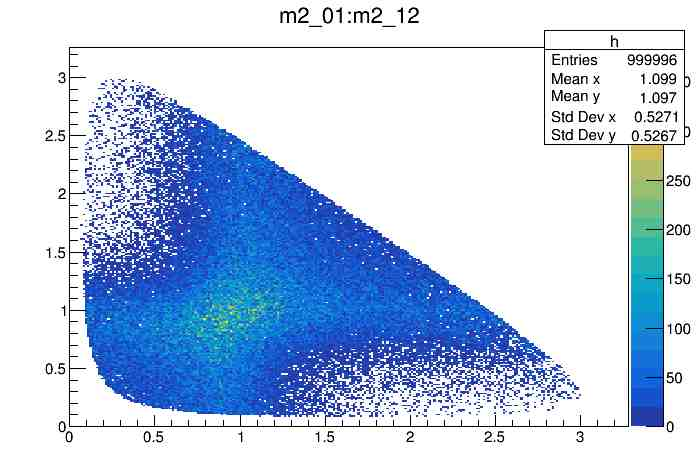
\includegraphics[width=.9\textwidth]{fig/toy_example.pdf}
    \caption{\ac{mc}-generated data set for testing the \ac{mipwa} approach in \ac{yap}.}
    \label{fig:mi_test_data}
\end{figure}



\begin{figure}
    \centering
    \begin{tikzpicture}
    \begin{axis}[
            error bars/y dir=both,
            error bars/y explicit,
            xlabel = {Bin index},
            ylabel = {Amplitude}
        ]
        \addplot+[ybar stacked] table [x index=0, y index=1, y error index=2] {data/output8bins/parameters.dat};
        %\addplot+[ybar stacked] table [x index=0, y index=1, y error index=2] {data/output8bins/parameters.dat};
    \end{axis}
\end{tikzpicture}

    \caption{Breit-Wigner fitted with eight equally-spaced bins using \ac{bat}.}
    \label{fig:mi_test_fit_amp_8bins}
\end{figure}

%----------------------------------------------------------------------------------------
% BACKMATTER
%
\backmatter
	% Acronyms
	\printnoidxglossaries

	% Index
	\cleardoublepage
	\phantomsection
	\addcontentsline{toc}{chapter}{\indexname}
	\printindex

	% Bibliography
	\cleardoublepage
	\phantomsection
	\addcontentsline{toc}{chapter}{\bibname}
	\nocite{*}
	\printbibliography

\end{document}
